% !TeX root = ../analisi_2.tex

\section{Integrali curvilinei}

\subsection{Definizione e proprietà}

\begin{definition}
Sia $f : A \subseteq \mathbb{R}^2 \to \mathbb{R}$, $A \neq \emptyset$, $A$ aperto, $f$ continua.

Sia $\gamma : [a, b] \to \gamma([a, b]) \subseteq A \subseteq \mathbb{R}^2$, regolare.

Si chiama \underline{integr. curvilineo} di $f$ lungo $\gamma$ il seguente
\[
\int_\gamma f \, ds = \int_a^b f(\gamma(t)) \vert \gamma'(t) \vert \, dt
\]
\end{definition}

\begin{center}
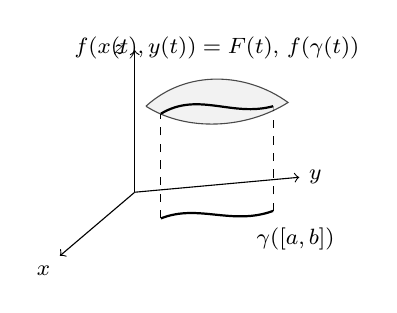
\begin{tikzpicture}[scale=0.95]
    % Assi 3D
    \draw[->] (0,0) -- (-1.0,-0.85) node[below left] {\footnotesize $x$};
    \draw[->] (0,0) -- (2.2,0.2) node[right] {\footnotesize $y$};
    \draw[->] (0,0) -- (0,1.9) node[left] {\footnotesize $z$};

    % Curva gamma([a,b]) nel piano xy
    \draw[thick] (0.35,-0.35) .. controls (0.85,-0.15) and (1.3,-0.45) .. (1.85,-0.25);
    \node[below right] at (1.5,-0.35) {\footnotesize $\gamma([a, b])$};

    % Proiezione verticale sulla superficie
    \draw[dashed] (0.35,-0.35) -- (0.35,1.05);
    \draw[dashed] (1.85,-0.25) -- (1.85,1.15);

    % Porzione di superficie f e curva sollevata
    \draw[fill=gray!15, opacity=0.7] (0.15,1.15) .. controls (0.7,1.65) and (1.5,1.6) .. (2.05,1.2) .. controls (1.5,0.85) and (0.7,0.8) .. (0.15,1.15);
    \draw[thick] (0.35,1.05) .. controls (0.85,1.35) and (1.3,1.0) .. (1.85,1.15);
    \node[above] at (1.1,1.65) {\footnotesize \pencilnote{$f(x(t), y(t)) = F(t)$, $f(\gamma(t))$}};
\end{tikzpicture}
\end{center}

\pencilnote{$\gamma$ può essere reg. a tratti.}

\begin{prop}[Es. obbligatorio]
Se $f : A \subseteq \mathbb{R}^2 \to \mathbb{R}$, $A \neq \emptyset$ e aperto e se $\gamma$ e $\psi$ sono 2 curve regolari con sostegno in $A$ t.c. $\gamma \sim \psi$ \pencilnote{($\gamma : [a, b] \to \mathbb{R}^2$, $\psi : [c, d] \to \mathbb{R}^2$)} allora
\[
\int_\gamma f \, ds = \int_\psi f \, ds
\]
\end{prop}

\begin{proof}
Per HP $\exists g \in C^1([c, d])$ \pencilnote{($g'(\tau) \neq 0$)} : $\psi(t) = \gamma(g(t))$ $\forall t \in [c, d] \implies \int_\psi f \, ds = \int_c^d f(\psi(t)) \vert \psi'(t) \vert \, dt$.

$\psi'(t) = \gamma'(g(t)) \cdot g'(t) \implies \vert \psi'(t) \vert = \vert \gamma'(g(t)) \vert \cdot \vert g'(t) \vert$, pongo $g(t) = \tau \to g'(t) \, dt = d\tau$ ottengo:
\begin{itemize}
    \item Se $g' > 0$:
    \[
    \int_a^b f(\gamma(\tau)) \vert \gamma'(\tau) \vert \, d\tau = \int_\gamma f \, ds = \int_\psi f \, ds
    \]
    \item Se $g' < 0$: ottengo:
    \[
    \int_c^d f(\gamma(g(t))) \vert \gamma'(g(t)) \vert \cdot (-g'(t)) \, dt = -\int_b^a f(\gamma(\tau)) \vert \gamma'(\tau) \vert \, d\tau = \int_a^b f(\gamma(\tau)) \vert \gamma'(\tau) \vert \, d\tau = \int_\gamma f \, ds = \int_\psi f \, ds
    \]
\end{itemize}
\end{proof}

\textbf{Proprietà:}
\begin{enumerate}
    \item \underline{Linearità}:
    \[
    \int_\gamma (\alpha f + \beta g) \, ds = \alpha \int_\gamma f \, ds + \beta \int_\gamma g \, ds
    \]
    \item \underline{Monotonia}:
    \[
    \text{Se } f \le g \implies \int_\gamma f \, ds \le \int_\gamma g \, ds
    \]
    \item \[
    \int_{\gamma_1 \cup \gamma_2} f \, ds = \int_{\gamma_1} f \, ds + \int_{\gamma_2} f \, ds \quad \text{\pencilnote{(additività su ``pezzi'' di curva)}}
    \]
    \item \[
    \left\vert \int_\gamma f \, ds \right\vert \le \int_\gamma \vert f \vert \, ds
    \]
    \item \[
    \int_\gamma 1 \, ds = l(\gamma)
    \]
\end{enumerate}

\subsection{Baricentro di una curva}

\begin{definition}
Sia $\gamma : [a, b] \to \mathbb{R}^2$ regolare e semplice e indichiamo con $\Gamma$ il suo sostegno; si chiama \underline{baricentro di $\Gamma$} è il punto $B = (x_B, y_B)$ dove
\[
x_B = \frac{1}{l(\gamma)} \int_\gamma x \, ds, \qquad y_B = \frac{1}{l(\gamma)} \int_\gamma y \, ds
\]
\end{definition}

\begin{example}[Calcolare il baricentro della cicloide]
\[
x_B = \frac{1}{l(\gamma)} \int_\gamma x \, ds \qquad y_B = \frac{1}{l(\gamma)} \int_\gamma y \, ds
\]
\[
\gamma : \begin{cases}
x(t) = r(t - \sin t) \\
y(t) = r(1 - \cos t)
\end{cases} \quad t \in [0, 2\pi], \ r > 0
\]
\[
\vert \gamma'(t) \vert^2 = 2r^2(1 - \cos t)
\]
\[
\begin{aligned}
l(\gamma)
&= \int_0^{2\pi} \sqrt{2r^2(1-\cos t)}\,dt \\[4pt]
&= 2r \int_0^{2\pi}
\sqrt{\frac{1-\cos t}{2}}\,dt \\[4pt]
&= 2r \int_0^{2\pi}
\underbrace{\sin\frac{t}{2}}_{\geq 0}\,dt \\[4pt]
&= 2r \left[-2\cos\frac{t}{2}\right]_0^{2\pi} \\[4pt]
&= 8r.
\end{aligned}
\]
\[
x_B = \frac{1}{8r} \int_0^{2\pi} \underbrace{r(t - \sin t)}_{x(t)} \underbrace{\sqrt{2}\, r \sqrt{1 - \cos t} \, dt}_{ds} = \frac{\sqrt{2}\, r}{8} \int_0^{2\pi} \left( t\sqrt{1 - \cos t} - \sin t \sqrt{1 - \cos t} \right) dt =
\]
\[
= \frac{r}{4} \left[ \int_0^{2\pi} t \sin\frac{t}{2} \, dt - \int_0^{2\pi} \underbrace{\sin t}_{2\cos\frac{t}{2}\sin\frac{t}{2}} \sin\frac{t}{2} \, dt \right] = \dots = \pi r
\]
\[
y_B = \frac{4}{3} r
\]
\end{example}

\subsection{Esempi di calcolo}

\begin{example}
Calcolare $\int_\gamma \left( x^2 + \frac{y}{\sqrt{x^2 + 1}} \right) ds$ dove $\gamma$ è il bordo della porzione di piano racchiusa dal grafico del $\log$ per $x \in [1, e]$ e dall'asse $x$.

\begin{center}
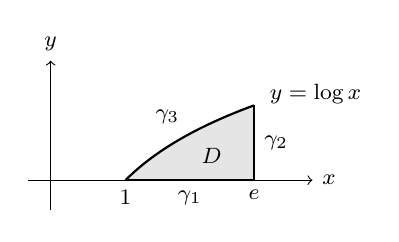
\begin{tikzpicture}[scale=0.95]
    % Regione D
    \fill[gray!20] (1,0) -- (2.718,0) -- (2.718,1) -- plot[domain=2.718:1, samples=40] (\x, {ln(\x)}) -- cycle;
    % Assi
    \draw[->] (-0.3,0) -- (3.5,0) node[right] {\footnotesize $x$};
    \draw[->] (0,-0.4) -- (0,1.6) node[above] {\footnotesize $y$};
    % Bordi gamma_1, gamma_2, gamma_3
    \draw[thick] (1,0) -- (2.718,0) node[midway, below] {\footnotesize $\gamma_1$};
    \draw[thick] (2.718,0) -- (2.718,1) node[midway, right] {\footnotesize $\gamma_2$};
    \draw[thick, domain=1:2.718, samples=40] plot (\x, {ln(\x)});
    \node[above left] at (1.85,0.62) {\footnotesize $\gamma_3$};
    \node[right] at (2.8,1.15) {\footnotesize $y = \log x$};
    \node[below] at (1,0) {\footnotesize $1$};
    \node[below] at (2.718,0) {\footnotesize $e$};
    \node at (2.15,0.32) {\footnotesize $D$};
\end{tikzpicture}
\end{center}

$\gamma = \gamma_1 \cup \gamma_2 \cup \gamma_3$
\[
\int_\gamma f \, ds = \int_{\gamma_1} f \, ds + \int_{\gamma_2} f \, ds + \int_{\gamma_3} f \, ds
\]
\[
\gamma_1 = \begin{cases}
x = t \\
y = 0
\end{cases} \quad t \in [1, e] \qquad \vert \gamma'_1(t) \vert = 1
\]
\[
\gamma_2 = \begin{cases}
x = e \\
y = t
\end{cases} \quad t \in [0, 1] \qquad \vert \gamma'_2(t) \vert = 1
\]
\[
\gamma_3 = \begin{cases}
x = t \\
y = \log t
\end{cases} \quad t \in [1, e] \qquad \vert \gamma'_3(t) \vert = \sqrt{1 + \frac{1}{t^2}}
\]
\[
\begin{aligned}
\int_\gamma f \, ds &= \int_1^e t^2 \, dt + \int_0^1 \left( e^2 + \frac{t}{\sqrt{1 + e^2}} \right) dt + \int_1^e \left( t^2 + \frac{\log t}{\sqrt{t^2 + 1}} \right) \frac{\sqrt{t^2 + 1}}{t} \, dt = \\
&= \left[ \frac{t^3}{3} \right]_1^e + \left[ e^2 + \frac{1}{\sqrt{1 + e^2}} \cdot \frac{1}{2} \right] + \left[ \frac{2}{3} \cdot \frac{1}{2} (1 + t^2)^{\frac{3}{2}} + \frac{\log^2 t}{2} \right]_1^e = \dots
\end{aligned}
\]
\end{example}
